
\chapter{Model Selection and Evaluations Metrics :}\label{descriptors}

\section{model selection}\label{variance_bias}
Model selection is the process of choosing between different machine learning approaches,  or choosing between different hyperparameters or sets of features for the same machine learning approach  like in LSTM  finding the right look back parameter, and the number of layers, nodes.
The choice of the actual machine learning algorithm is less important than we'd think  there may be a "best" algorithm for a particular problem, but often its performance is not much better than other well performing approaches for that problem.

There may be certain qualities we look for in an model:
\begin{itemize}
\item Interpretable   can we see or understand why the model is making the decisions it makes?
\item Accurate
\item Fast (to train and test)
\item Scalable (it can be applied to a large dataset)
\end{itemize}
Though there are generally trade offs among these qualities.\\in order to select a model from other models, we usually use one of the following approaches.\\\textbf{A Typical approach } is to take your data and split it randomly into a training set and a test set (e.g. a 70\%/30\% split). Then you train your model on the training set and see how it performs on the test set.\\The problem with this approach is that it results in an overly optimistic estimation of generalization if we tune our model's parameters with it,  so what we want to do instead is splitting the data is to not split it only into training and testing sets, but to also include a validation set. A typical ratio is 60\% training, 20\% validation, 20\% testing.

This way we can measure validation error instead of just measuring the test error .
We can use these errors   to identify what kind of problem we have if our model isn't performing well:

\begin{itemize}
\item If our training error is large and our validation/test set error is large, then we have a high bias (underfitting) problem.
\item If our training error is small and our validation/test set error is large, then we have a high variance (overfitting) problem.
\end{itemize}
As the figure \ref{fig:bias} explains : 
\begin{figure}[H]
\centering
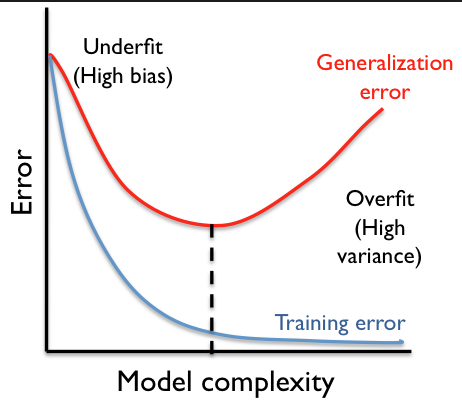
\includegraphics[width=0.38\textwidth]{img/model.png}
\caption{ bias / variance Tradeoff}
\label{fig:bias}
\end{figure}
Some ways of evaluating a model's performance on (some of)  known data are for \textbf{validation set } to pick  the best model you can possibly get :
\begin{itemize}
\item Hold out (just set aside some portion of the data for validation; this is less reliable if the amount of data is small such that the held out portion is very small) 
\item K-fold cross-validation (better than hold out for small datasets) for better visualization  check figure \ref{fig:cross}
%
\begin{itemize}
\item The training set is divided into k folds
\item Iteratively take k-1 folds for training and validate on the remaining fold
\item Average the results
\item There is also "leave-one-out" cross-validation which is k-fold cross-validation where k=n (n is the number of data points)
\end{itemize}
%
%
\begin{figure}[H]
\centering
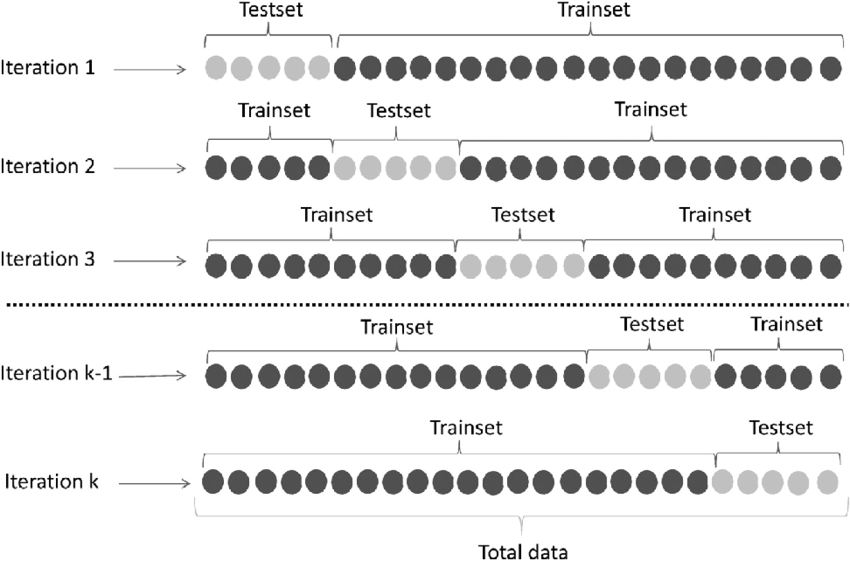
\includegraphics[scale=0.9]{img/cross.png}
\caption{K-cross validation }
\label{fig:cross}
\end{figure}
%
\item Bootstrapping : 
\begin{itemize}
\item New datasets are generated by sampling with replacement (uniformly at random) from the original dataset
\item Then train on the bootstrapped dataset and validate on the unselected data
\end{itemize}
\end{itemize}
%
\subsection{Evaluating classification models}\label{eva}
Every model comes with parameters that can modify the model's behavior and performance, evaluation of the model  often comes in the form of a confusion matrix \ref{confu}.
% Please add the following required packages to your document preamble:

% Please add the following required packages to your document preamble:
% \usepackage{multirow}
\begin{table}[]
\centering
\caption{Confusion matrix}
\label{confu}
\begin{tabular}{lllclll}
\cline{3-4}
                                                                                                        & \multicolumn{1}{l|}{}           & \multicolumn{2}{l|}{\textbf{Predicted Class}}                                                                                                                                                            &                               &  &  \\ \cline{3-4}
                                                                                                        & \multicolumn{1}{l|}{}           & \multicolumn{1}{l|}{\textbf{P}}                                                                    & \multicolumn{1}{l|}{\textbf{N}}                                                                     &                               &  &  \\ \cline{1-4}
\multicolumn{1}{|l|}{\multirow{2}{*}{\textbf{\begin{tabular}[c]{@{}l@{}}Actual \\ Class\end{tabular}}}} & \multicolumn{1}{l|}{\textbf{P}} & \multicolumn{1}{l|}{\textbf{\begin{tabular}[c]{@{}l@{}}True Positives\\        (TP)\end{tabular}}} & \multicolumn{1}{l|}{\textbf{\begin{tabular}[c]{@{}l@{}}False Negatives\\        (FN)\end{tabular}}} & \multicolumn{1}{c}{\textbf{}} &  &  \\ \cline{2-4}
\multicolumn{1}{|l|}{}                                                                                  & \multicolumn{1}{l|}{\textbf{N}} & \multicolumn{1}{c|}{\textbf{\begin{tabular}[c]{@{}c@{}}False Positives\\ (FP)\end{tabular}}}       & \multicolumn{1}{c|}{\textbf{\begin{tabular}[c]{@{}c@{}}True Negatives\\ (TN)\end{tabular}}}         & \textbf{}                     &  &  \\ \cline{1-4}
                                                                                                        &                                 & \multicolumn{1}{c}{\textbf{}}                                                                      & \textbf{}                                                                                           & \multicolumn{1}{c}{\textbf{}} &  &  \\
                                                                                                        &                                 & \multicolumn{1}{c}{\textbf{}}                                                                      & \textbf{}                                                                                           & \multicolumn{1}{c}{\textbf{}} &  & 
\end{tabular}
\end{table}


The core values are:
\begin{itemize}
\item True positives (TP): samples classified as positive which were labeled positive
\item True negatives (TN): samples classified as negative which were labeled negative
\item False positives (FP): samples classified as positive which were labeled negative
\item False negatives (FN): samples classified as negative which were labeled positive
\end{itemize}

here is some important quantities we need to know in order to evaluate a model :
\begin{itemize}
\item Recall  also known as True Positive Rate (TPR): $ \frac{TP}{TP+FN}$ 
\item False Positive Rate (FPR): $\frac{TN}{TN+FP}$
\item Positive predictive value:  $\frac{TP}{TP+FP}$ 
\item Negative predictive value: $\frac{TN}{TN+FN}$
\item Precision: How many of the predicted positive samples are correctly predicted   $\frac{\text{TP}}{\text{TP} + \text{FP}}$

\item Accuracy : $\frac{TP+TN}{TP+FP+TN+FN}$

\item The F-score is often introduced as harmonic mean of precision and recall.

$F$-$score= \frac{\text{2} \cdot \text{Precision } \cdot \text{ Recall} }{ \text{Precision} + \text{ Recall}}$
\end{itemize}


\subsection{Performance measures}
Final parameter selection and performance were measured by Mean Absolute Error (MAE) given by 
%
\begin{equation}
\label{eq:MAE}
MAE = \frac{1}{n}\sum^{n}_{i=1} \left | y_{obs_{i}}- y_{pred_{i}} \right |
\end{equation}
%
and Root Mean Square Error given by
%
\begin{equation}
\label{eq:RMSE}
RMSE = \sqrt{\frac{1}{n}\sum^{n}_{i=1} \left ( y_{obs_{i}}- y_{pred_{i}} \right )^{2}}
\end{equation}
MAE and RMSE are widely used measures of continuous variables with RMSE criticized for over-biasing towards large errors \cite{Chai2014Willmott2005}. Both metrics were calculated for comparison; however MAE is used more often for descriptive analytics.
\subsubsection{Area under the ROC curve (ROC AUC)}
Receiver Operating Characteristics  ( ROC) is a method that visualizes, organizes and selects models based on  their performance,  this method is for binary classification, but we can adapt it to multi-classification problem  using "OneVsAll" approach, it basically  visualizes the performance of our classifier through all the thresholds, whereas accuracy and F-score  metrics, etc, judge the performance based on particular threshold (usually  0.5) above this cut-off one label is assigned, and below it the other label is assigned. But  looking at all thresholds at once, can give a clear and more honest image of the real performance of our classifier,  since  some models may work best with a different threshold and data sometimes can be biased,   that's when  a dataset has way more or way less of the positive class than there are of the negative class. This imbalance in data can give deceptive and false results if we used accuracy as a metric, to clear the idea more let's say we have a dataset of 100 training example in which it  has 99 example positive and 1 negative example.  The accuracy here can be very deceptive with a value of 99\% so accuracy can't tell much here, the F$\textbf{-}$score can take  into consideration these kind of unbalanced data,  by considering  the true \textbf{positive } rate and the true \textbf{predictive} value  but  it does  not consider all the thresholds of the classifier. However  ROC  is insensitive to bias data ( unbalanced data ) and can run over all thresholds and plots, the  true vs false positive rates, varying the threshold can give us pair of (FPR,TPR) \ref{fig:bias2}.
\begin{figure}[H]
\centering
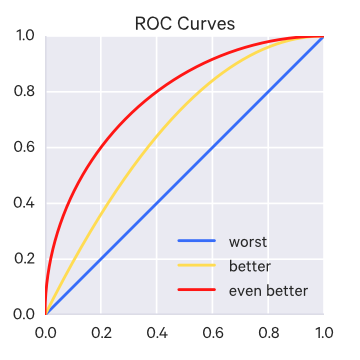
\includegraphics[width=0.45\textwidth]{img/roc.jpg}
\caption{ ROC curve }
\label{fig:bias2}
\end{figure}
The area under the curve (AUC) is used to quantify how good the classifier is. The AUC is in fact  the probability that a classifier will rank a randomly chosen positive instance higher than a randomly chosen negative one, (assuming 'positive' ranks higher than 'negative'). Generally, an AUC of above 0.8 is considered "good", an AUC of 0.5 (a straight line) is equivalent to random guessing.


\section{Conclusion:}

In this chapter we have presented in detail some of the most popular  methods for selecting  a model using K-fold cross validation, and their astonishing role in maximizing the performance of a classifier by choosing the optimal hyperparameters of a model.
Finally we reviewed  how to  assess the performance of a fully trained classifier using area under ROC curve ( ROC AUC ).
In the next chapter we will finally take a look on the techniques used for imputation, and we will discuss multiple results.
